\section{Resultados Obtidos}

Os resultados compreendem as etapas de avalização e implantação do CRISP-DM. Nesta seção, apresentamos os resultados obtidos com a análise dos dados da RAIS. De uma maneira geral, as análises compreendem homens e mulheres no setor de TI no Brasil ao longo dos anos. 

Para as análises das subseções \ref{sub:geral}, \ref{sub:educ}, \ref{sub:privpub}, criamos dois gráficos, um com a quantidade de pessoas e outro com a média salarial. As linhas de cor rosa são relacionadas a mulheres e as de azul são relacionadas a homens. As porcentagens exibidas na linha das mulheres são relativas ao valor corresponente na do homem no mesmo ano. 

\subsection{Análise com uma visão geral dos dados} \label{sub:geral}

\subsubsection{Quantidade}

Vemos que no primeiro gráfico da Figura \ref{fig_1_qnt}, a quantidade de homens é maior que a de mulheres, uma situação já esperada. É importante destacar a diferença em 2021 de -74,78\% para mulheres, a maior diferença entre todos os anos. Além do mais, 2021 foi um ano de pandemia, o que pode ter influenciado nesse resultado.

\begin{figure}[htbp]
	{
		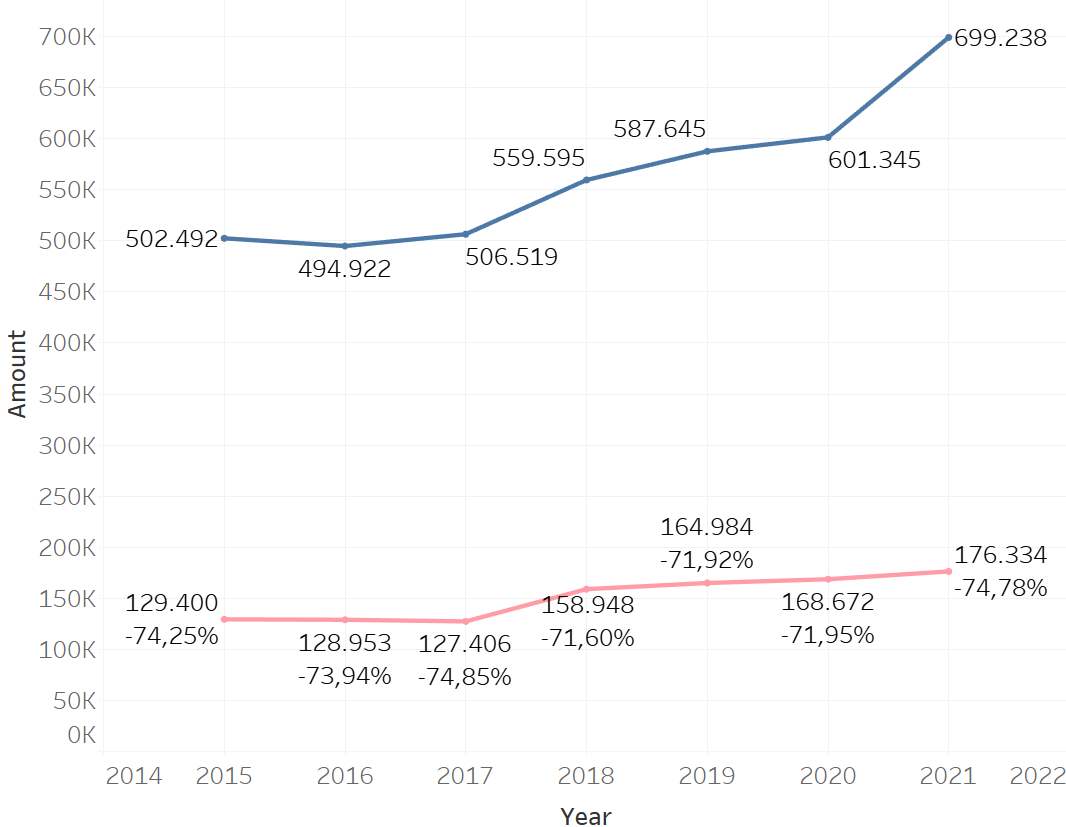
\includegraphics[width=85mm]{assets/1_qnt.PNG}
	}
	\caption{Quantidade geral}
	\label{fig_1_qnt}
\end{figure}

\subsubsection{Média salarial}

No segundo gráfico da Figura \ref{fig_1_sal}, vemos que a média salarial dos homens é maior que a das mulheres, porém para o período de 2018 a 2020 há um aumento na diferença entre os gêneros. Em 2021, a diferença diminuiu entre os sexos, e ainda, tanto o homem quanto a mulher tiveram um aumento na média salarial. Nossa suposição é de que, com a pandemia, o aumento do teletrabalho tenha proporcionado a valorização dos profissionais de TI.

\begin{figure}[htbp]
	\centerline{
		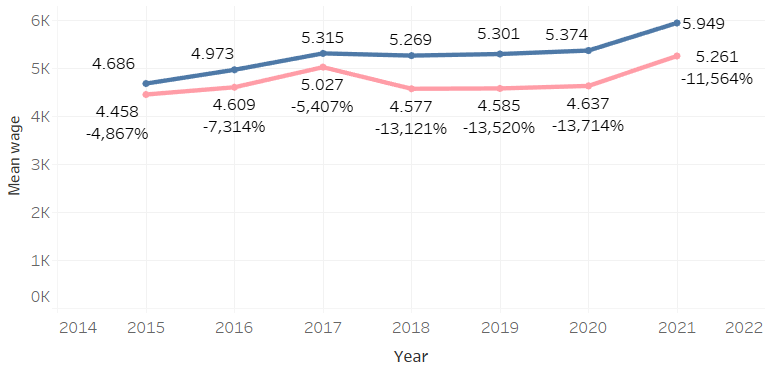
\includegraphics[width=85mm]{assets/1_sal.PNG}
	}
	\caption{Média salarial geral}
	\label{fig_1_sal}
\end{figure}


\subsection{Por nível educacional}  \label{sub:educ}

\subsubsection{Quantidade}

Em uma análise educacional, conforme a Figura \ref{fig_2_qnt_educ}, percebemos nos dois gêneros que há um número maior de pessoas com ensino superior em contraste às com ensino médio completo. É interessante notar que, em 2021, a diferença relativa entre os gêneros é bem próxima para o os dois níveis escolares (na casa dos 73,22\%).

\begin{figure}[htbp]
	\centerline{
		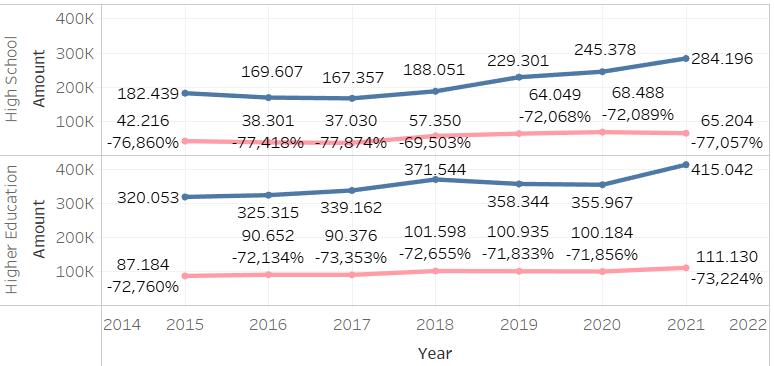
\includegraphics[width=85mm]{assets/2_qnt_educ.PNG}
	}
	\caption{Quantidade por nível educacional}
	\label{fig_2_qnt_educ}
\end{figure}

\subsubsection{Média salarial}

Para média salarial da Figura \ref{fig_2_sal_educ}, vemos que a diferença é maior para nível médio (-23,27\%) em 2021, enquanto que para o superior é de -11,25\%. Ou seja, a diferença é mais do que o dobro quando olhamos para o salário e o nível médio. Com isso, podemos supor que a qualificação da mulher ajuda a reduzir a desigualdade salarial na TI.

\begin{figure}[htbp]
	\centerline{
		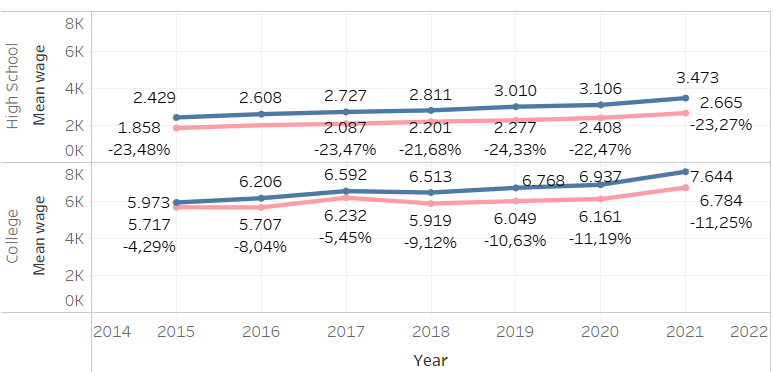
\includegraphics[width=85mm]{assets/2_sal_educ.PNG}
	}
	\caption{Média salarial por nível educacional}
	\label{fig_2_sal_educ}
\end{figure}

\subsection{Por setor Privado e Público}  \label{sub:privpub}

\subsubsection{Quantidade}

Na Figura \ref{fig_3_qnt_pubpriv} abaixo é nítida a quantidade esmagadora de profissionais da área privada em relação à pública. Na Figura  \ref{fig_3_1_qnt_pubpriv} nós ampliamos a imagem, já que fica difícil de visualizar a diferença entre os gêneros.

\begin{figure}[htbp]
	\centerline{
		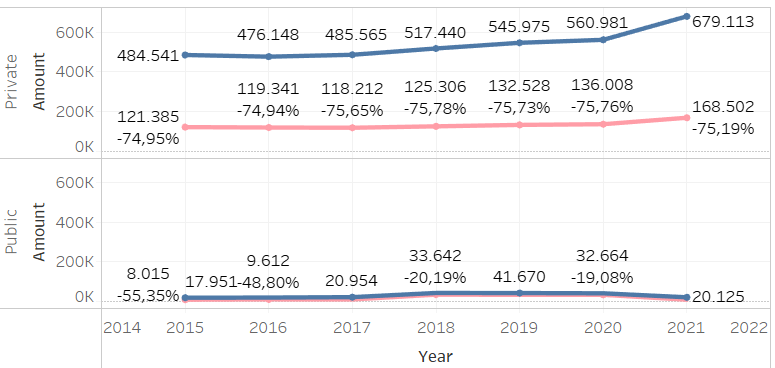
\includegraphics[width=85mm]{assets/3_qnt_pubpriv.PNG}
	}
	\caption{Quantidade por setor}
	\label{fig_3_qnt_pubpriv}
\end{figure}


\begin{figure}[htbp]
	\centerline{
		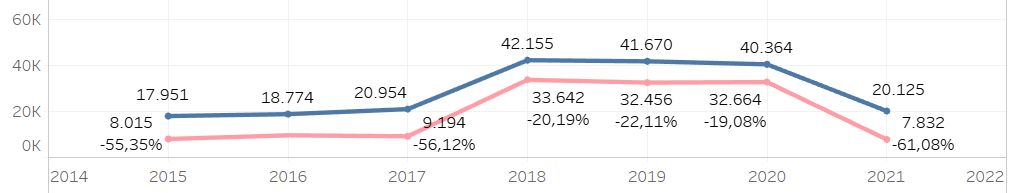
\includegraphics[width=85mm]{assets/3_1_qnt_pubpriv.PNG}
	}
	\caption{Gráfico ampliado da quantidade por setor público}
	\label{fig_3_1_qnt_pubpriv}
\end{figure}

\subsubsection{Média salarial}

Para o setor privado da Figura \ref{fig_3_sal_pubpriv}, fica visível a diferença entre os gêneros, sendo para 2021 de -13\%, que em termos absolutos é de 796 reais. Para um padrão brasileiro, essa diferença é grande, pois representa quase um salário mínimo (R\$ 1.100 em 2021)\footnote{https://www.congressonacional.leg.br/materias/medidas-provisorias/-/mpv/146145}. Já para o setor público a diferença é bem pequena, com exceção para os anos de 2018 a 2021, algo já previamente destacado na média geral da Figura \ref{fig_1_sal}.

\begin{figure}[htbp]
	\centerline{
		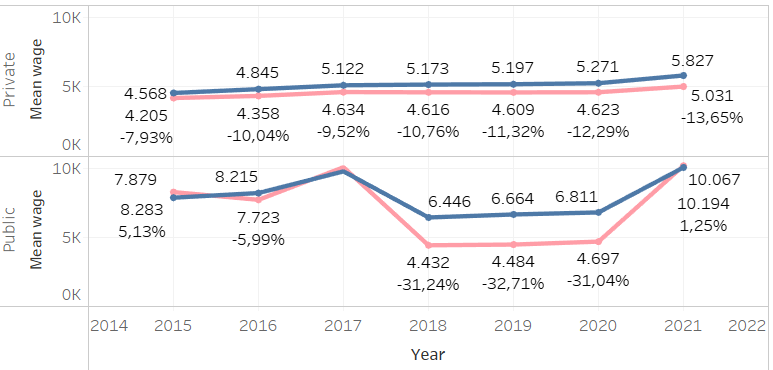
\includegraphics[width=85mm]{assets/3_sal_pubpriv.PNG}
	}
	\caption{Média salarial por setor}
	\label{fig_3_sal_pubpriv}
\end{figure}

\subsection{Quantidade de demissões}

Esta seção analisa de forma diferente das anteriormente expostas. Há um gráfico para cada gênero. Em cada gráfico, há a quantidade de pessoas demitidas e, logo abaixo, a de pessoas não demitidas, ou seja, mantidas no emprego no respectivo ano. A porcentagem é também diferente, pois analisa a diferença em relação ao dado anterior da própria linha, e não em relação ao outro sexo.

\subsubsection{Homem}

Destacamos aqui na Figura \ref{fig_4_qnt_h_demit} que o aumento de 35,82\% em 2021 foi o maior entre os outros anos. Isso mostra que a quantidade de demissões aumentou muito em relação ao ano anterior, que era de 116.604 demissões. 

\begin{figure}[htbp]
	\centerline{
		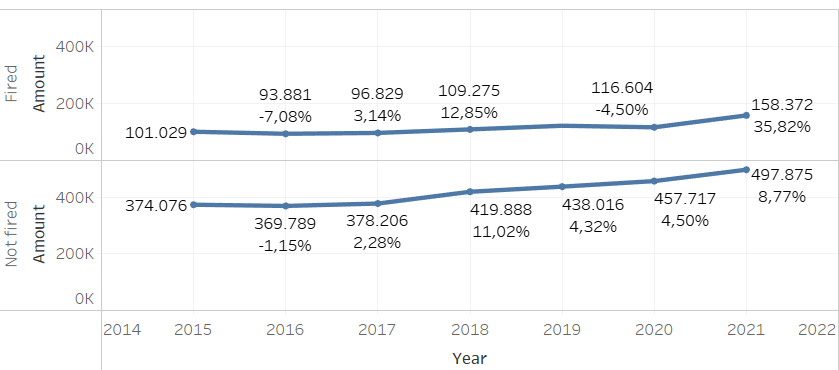
\includegraphics[width=85mm]{assets/4_qnt_h_demit.PNG}
	}
	\caption{Demissões de homens}
	\label{fig_4_qnt_h_demit}
\end{figure}

\subsubsection{Mulher}

Na Figura \ref{fig_4_qnt_m_demit}, é perceptível o mesmo aumento do gráfico anterior, porém com uma porcentagem de 29,91\% em relação a 2020. O grande número de demissões acontece em um ano em que a pandemia ainda estava em vigor. 

\begin{figure}[htbp]
	\centerline{
		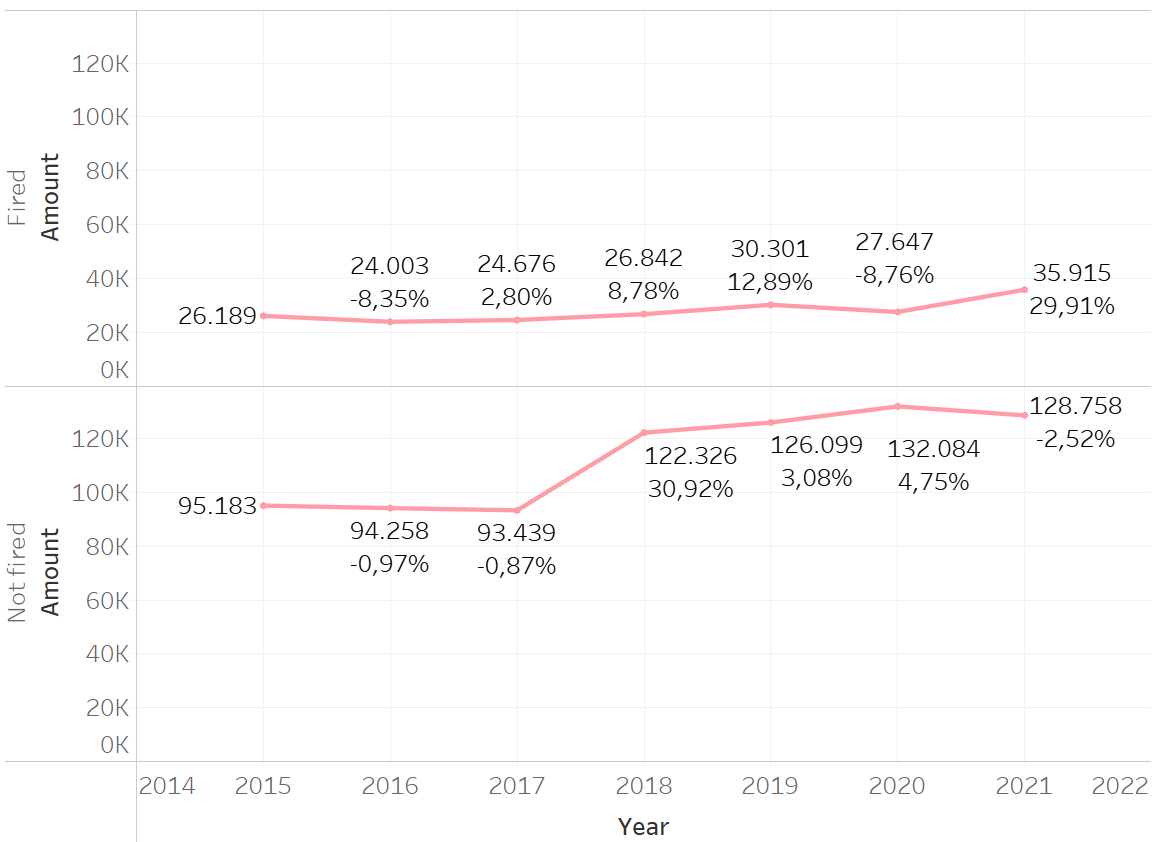
\includegraphics[width=85mm]{assets/4_qnt_m_demit.PNG}
	}
	\caption{Demissões de mulheres}
	\label{fig_4_qnt_m_demit}
\end{figure}

\subsection{Por cargo de TI}

Nas análises por cargos abaixo, consideramos apenas o ano de 2021, pois é o último ano disponível em nossa análise.

\subsubsection{Quantidade}

Podemos ver na Figura \ref{fig_5_qnt_cbo} abaixo que a quantidade de Analistas de Desenvolvimento de Sistemas é a que concentra a maior quantidade de profissionais, seguido por Analistas de Suporte Computacional, isso em ambos os sexos. 

\subsubsection{Média salarial}

Já na Figura \ref{fig_5_sal_cbo} é visível a diferença de salário entre o cargo com maior média e os demais. Portanto, para o cargo de Engenheiros de Sistemas Operacionais em Computação, há uma diferença de mais de 1.000 reais entre os sexos. Porém há um dado curioso, no cargo de Analista de Redes e de Comunicação de Dados há um ligeiro ganho salarial para as mulheres. Enquanto que para os homens é de 6.233 reais, para as mulheres é de 6.270 reais, ou seja, uma diferença de 2,17\% a mais para as mulheres.

\begin{figure}[htbp]
	\centerline{
		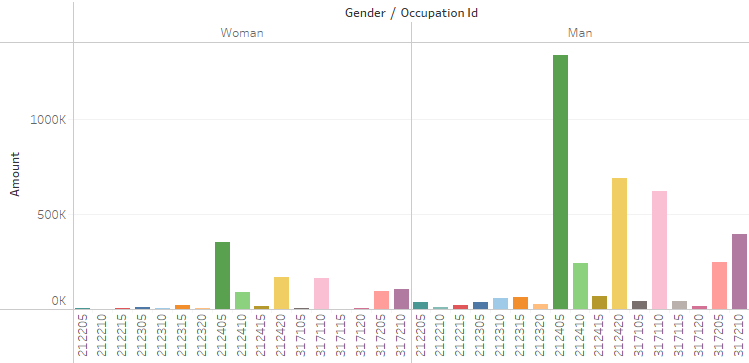
\includegraphics[width=85mm]{assets/5_qnt_cbo.PNG}
	}
	\caption{Quantidade por cargo em 2021}
	\label{fig_5_qnt_cbo}
\end{figure}

\begin{figure}[htbp]
	\centerline{
		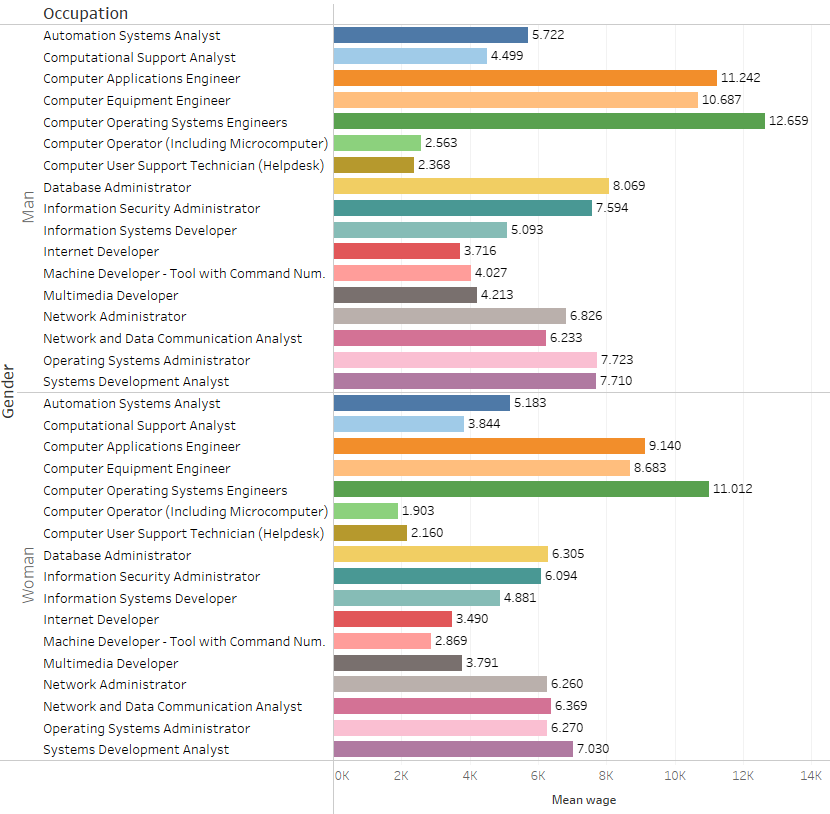
\includegraphics[width=85mm]{assets/5_sal_cbo.PNG}
	}
	\caption{Média salarial por cargo em 2021}
	\label{fig_5_sal_cbo}
\end{figure}